\documentclass[]{aastex62}
\usepackage{amssymb,amsmath}

 
\newcommand{\vk}{von K\'{a}rm\'{a}n}
\newcommand{\vdag}{(v)^\dagger}
\newcommand\aastex{AAS\TeX}
\newcommand\latex{La\TeX}


\def\eq#1{\begin{equation} #1 \end{equation}}
\def\mic              {\hbox{$\mu\mathrm{m}$}}
\def\atm    {\hbox{\rm{ATM}}}

\graphicspath{{./}{figures/}}
 
\shorttitle{Hot and Cold SOC-i Cases}
\shortauthors{Tate \& Ivezi\'{c}}

\begin{document}

\title{Hot and Cold Cases for Perun Thermal Analysis (v1)}  
 
%\email{ivezic@uw.edu}

\author{Perun Thermal Analysis Group}
\affiliation{Adriatic Aerospace Association}

\begin{abstract}
We computed temperature variation with time for the Perun satellite using a variety of input
assumptions. The computation is based on a simple model for the satellite temperature variation 
with time when the satellite is subjected to a bistable heat source: two orbital segments with 
piece-wise constant power. The model assumes that at a given time a single temperature applies 
to the entire satellite body. 
We defined the so-called ``hot'' and ``cold'' cases and found that the low and high temperature 
extremes for a randomly oriented Perun satellite are $-$14 $^\circ$C and $+$17 $^\circ$C. When the 
satellite orientation is deliberately chosen to maximize the temperature extremes, the corresponding 
values are $-$38 $^\circ$C and $+$42 $^\circ$C. These results, and the allowed operating temperature
ranges for satellite components imply that low temperatures will be more worrisome than high
temperatures. We also explored a toy model for active temperature control that assumes an additional
internal power dissipation whenever the satellite temperature drops below a pre-defined threshold,
and concluded that such an approach is a viable method for mitigating low temperatures.
These results are sensitive to assumed specific heat, which we simply assumed to correspond to 
aluminum, and should be revisited with more accurate input values. 
\end{abstract}

\keywords{Satellites --- CubeSat --- Perun --- Radiative transfer --- Thermal model}


\section{Introduction}
 
When designing a satellite such as Perun, it is crucial to establish that the temperature variation for 
each component will be within its operating range. In practice, professional engineering tools and 
numerical analysis are used to analyze complex systems. The Perun team utilizes the code Ansys
to predict satellites temperature distribution. In order to compute temperatures, Ansys requires
as input numerical specifications for the sources of radiation that Perun absorbs. In addition, 
the satellite's orbital parameters and orientation are also required. Given that the details of 
Perun orbit will not be known until its launch, here we define the so-called ``hot'' and ``cold'' 
cases which capture scenarios that predict the coldest and the hottest satellite temperatures. 
 
In addition, we computed Perun temperature variation with time for hot and cold cases using
a simple model that assumes that a single temperature applies to the entire satellite body 
at any given time. Although simple, this modeling produces approximately correct temperature
estimates and deep physical insight, and can be used for fast studies of the impact of various
input assumptions on the resulting satellite temperature. Most importantly, these results 
provide a ``sanity check'' for the more sophisticated, but also more prone to input errors, 
Ansys models.
 
The main quantitative result of the models presented here is that it is much more likely 
for low than for high temperatures to present problems for Perun operations phase. 
Motivated by this finding, we also explored a toy model for active temperature control that 
assumes an additional internal power dissipation whenever the satellite temperature
drops below a pre-defined threshold. 

In the next section, we first describe our mathematical model and input parameters, and then 
discuss specific results obtained with input parameters corresponding to Perun. In \S\ref{sec:active},
we present a toy model for active temperature control, and summarize our findings in \S\ref{sec:conclusions}. 



\section{Thermal Analysis for Perun} 

The mathematical model for thermal analysis is discussed in detail in an accompanying document 
(\v{Z}. Ivezi\'{c}, 2021, unpublished, hereafter I21).  Here we extend analysis from a bistable heat source
discussed there to an arbitrary heating pattern along the orbit, including a temperature-driven
additional internal power dissipation. For this reason, we had to resort to a numerical solution
of the governing differential equation (see eq.~1 in I21, hereafter I21-eq1). A sufficient accuracy of numerical 
solution was verified using analytic solution for a case with piecewise constant bistable heat source (I21-eq17). 

Model input parameters include environmental, orbital and satellite parameters, all of them
subject to appreciable uncertainties. At least in principle, orbital and satellite parameters 
are deterministic and should not have any uncertainties. However, detailed orbital information
is sometimes unknown until the launch, and satellite orientation might be subject to 
operational uncertainties. We first describe Perun physical parameters used in computations
here, and then discuss orbital and environmental parameters, including definitions of the 
so-called ``hot'' and ``cold'' cases that attempt to account for various modeling uncertainties. 
After all the input parameters are introduced, we discuss the results of thermal modeling. 
 

\subsection{Input satellite parameters}

We used the Perun CAD model developed for structural analysis to extract information about
external satellite surfaces and their material properties. We adopted the following description 
of external Perun surfaces: 
\begin{itemize}
\item  Top: 60\% solar panel, 40\% aluminum frame
\item  Bottom: 38\% aluminum frame, 62\% PCB (printed circuit board). 
\item  Sides (2): 64\% solar panels, 19\% aluminum panels (outside), 17\% aluminum frame rails
\item  Sides (2): 57\% solar panels, 26\% aluminum panels (outside), 17\% aluminum frame rails
\end{itemize}

With the values of absorptivity and emissivity listed in Table~\ref{tab:inputsAbsEmiss}, we obtained
their surface-weighted values $\alpha=0.83$ and $\epsilon=0.79$ (54\% of external surface area
is covered by solar panels). In addition, we assumed that the satellite mass is $m=2.6$ kg and 
adopted specific heat corresponding to aluminum ($C=768$  J\,kg$^{-1}$\,K$^{-1}$), yielding a
thermal intertia of $mC = 2.00$ kJ\,K$^{-1}$. This value of thermal intertia needs to be verified with 
detailed modeling (e.g., summing the $mC$ product for all individual structural components
in the Perun CAD model). 

\begin{table}[t]
	\centering
	\caption{Surface optical absorptivity and infrared emissivity for Perun surface materials. }
	\label{tab:inputsAbsEmiss}
	\begin{tabular}{r|r|r|r|r|r} % 
		\hline
  	              Part        &                Surface          &    $\alpha$  &   $\epsilon$    &   $k$ (W\,m$^{-1}$\,K$^{-1}$)   &  $C$ (J\,kg$^{-1}$\,K$^{-1}$)  \\
	  	\hline
         Solar panels        &       GaAs, with AR coating  &           0.92      &          0.85      &   60.6    &      324   \\  
     Al panels, outside   &     7075 Al, Kapton             &           0.87       &         0.81       &  121.2   &    801   \\ 
          Al frame rails    &       5052 Al, hard anodized &          0.86        &        0.86      &    138.5   &    768    \\  
                Al frame      &       5052 Al, alodine            &          0.08        &        0.15       &   138.5   &    768    \\
                PCBs            &               FR4                        &           0.81       &         0.90        &   18.0  &    1544  \\ 
 		\hline     
	\end{tabular} 
\end{table}
 

\subsection{Assumptions for orbital parameters}

It is already known that Perun will have a nearly-polar sun-synchronous 
orbit\footnote{See https://en.wikipedia.org/wiki/Sun-synchronous\_orbit} 
with an altitude of $h=550$ km and orbital inclination of 97.7 degrees. A satellite in sun-synchronous 
orbit passes over any given point of the planet's surface at the same local mean solar time because the 
orbit precesses through one complete revolution each year (that is, the orbit always maintains the same 
relationship with the Sun). 

The eclipse duration for sun-synchronous orbits depends on their right ascension of the 
ascending node (RAAN), which will not be known until the launch date (RAAN is determined
by the exact launch time). The orbital period for sun-synchronous orbit with an altitude of 
$h=550$ km is 96 mins, and the maximum eclipse duration is 36 mins.  When the orbital 
plane is perpendicular to incoming solar radiation, there is no eclipse (the satellite is following 
the terminator line at all times). 


\begin{table}[t]
	\centering
	\caption{The range of input enviromental parameters. }
	\label{tab:inputsEnvParam}
	\begin{tabular}{r|r|r|r|r} % 
		\hline
  	         Quantity & max    &   min   &  mean &  unit            \\
		\hline
              Solar flux   &  1422  &  1322  &  1372 & Wm$^{-2}$  \\
           Earth albedo  &    35    &    25    &     30  &   \%            \\ 
            Earth IR flux &  260    &   220   &    240 & Wm$^{-2}$   \\
 		\hline
	\end{tabular} 
\end{table}


\subsection{The concept of hot and cold cases} 

Due to uncertainties in input parameters, including environmental, orbital and satellite parameters,
engineering pre-launch analysis often focuses on most extreme scenarios that predict the coldest 
and the hottest satellite temperatures. We define ``hot'' and ``cold'' cases by first adopting 
the extreme values of environmental parameters from Table~\ref{tab:inputsEnvParam}. 

In addition, we make an assumption that the orientation of Perun's sun-synchronous orbit
results in an eclipse with maximum duration (36 min) for cold case, and no eclipse at all for 
hot case. 

The intensity of solar radiation reflected from Earth varies along the orbit (I21-eq6). For a polar 
orbit passing through subsolar point, $f_{alb}=0.62$ for the non-eclipsed part of the orbit, while 
for a polar orbit aligned with the terminator (with no eclipse), $f_{alb}=0.06$. Therefore, 
we adopt $f_{alb}=0.62$ for hot case and $f_{alb}=0.06$ for cold case (note that reflected solar 
radiation contributes more flux for cold case, when not in eclipse). 
 
With these assumptions, we use equations 3--13 from I21 to compute incoming heating flux.
For cold case, the only heating flux during the eclipsed portion of the orbit is IR flux from Earth. 
The variation of flux between hot and cold cases for three main heat sources is summarized in 
Table~\ref{tab:inputflux}. Note that reflected solar flux is smaller for hot case but this difference
is compensated by the absence of eclipsed orbital portion in hot case. 

Table~\ref{tab:inputflux} lists absorbed flux per unit area, assuming Perun's effective 
absorption coefficient ($\alpha$). {\bf The listed value are also appropriate for detailed 
Ansys-based modeling, but need to be corrected for $\alpha$ of each surface material.} 
The actual absorbed power (absorbed energy per unit time) depends on 
the values of $\eta_S$ and $\eta_E$, which in turn depend on orientation. We make additional 
assumptions about satellite orientation, as discussed next. 

\begin{table}[t]
	\centering
	\caption{Absorbed flux ($\alpha=0.83$) for hot and cold cases (in  Wm$^{-2}$). }
	\label{tab:inputflux}
	\begin{tabular}{r|r|r|r} % 
		\hline
  	                    Quantity  & hot case   &   cold  case &   ratio hot/cold    \\
		\hline
              Direct solar flux    &    1181        &     1098         &     1.08       \\
           Reflected solar flux  &     21.0        &     144.2        &     0.15     \\    
                       Earth IR flux  &   174.6       &     147.8        &     1.18      \\
		\hline
	\end{tabular} 
\end{table}



\subsection{Assumptions for satellite orientation}

The satellite orientation determines effective surface areas for the absorption of radiation from 
the Sun and Earth. For convenience, these surface areas are expressed relative to the total surface area, $A_{tot}$
(=0.1 m$^2$ for Perun), using $\eta$ factors ($\eta_S$ and $\eta_E$, respectively). For a given 
orbit and satellite orientation, $\eta_S$ and $\eta_E$ can be computed by adding corresponding
values (known as ``view factors'') for six individual sides (see Appendix A in I21).  

We used results discussed in Section 2.4 from I21 to adopt the following values for Perun.
When averaged over plausible orientations and orbits, $\eta_S = 0.21$ and $\eta_E = 0.36$, 
with an uncertainty due to actual orbit specifics of the order 10\%. The limits of 
possible ranges are  $\eta_S = 0.10 - 0.30$ and $\eta_E = 0.34 - 0.38$. The limits for 
$\eta_S$ reflect the range of projected area towards plane-parallel rays for 2U CubeSat geometry, 
with the minimum value corresponding to one small side oriented perpendicularly to the incoming 
solar radiation. For $\eta_E$, the variation is much smaller because typically all six sides can 
``see'' Earth's surface\footnote{We note that even for spherical geometry $\eta_S$ and $\eta_E$
are generally different:  $\eta_S=1/4$, while $\eta_E$ decreases from 1/2 to 1/4 as the orbit
altitude varies from zero to infinity.}. 
 
We do not adopt specific satellite orientation for hot and cold cases but instead explore two 
options in each case.  First, we adopt averaged orientations for both hot and cold cases,
with $\eta_S = 0.21$ and $\eta_E = 0.36$ corresponding to 2U CubeSat values. As the second 
assumption, we consider the following extreme cases: $\eta_S = 0.30$ and $\eta_E = 0.34$ for 
hot case, and $\eta_S = 0.10$ and $\eta_E = 0.38$ for cold case.  
 
The second set of values assumes that the satellite orientation is actively controlled.  For hot
case, the maximum possible projected satellite area for plane-parallel rays is always pointing 
towards the Sun ($\eta_S = 0.30$). For cold case and during non-eclipsed portion, the smallest 
satellite side is always pointing towards the Sun ($\eta_S = 0.10$).  The adopted values of 
$\eta_E$ are its extreme values. 



\newpage
\subsection{Assumptions for internal power dissipation}


A fraction of absorbed optical flux (the sum of direct solar flux and reflected solar flux) is often 
used to charge on-board batteries. We assume that 20\% of absorbed flux\footnote{Here, $\eta_{cell}$ 
represents the fraction of all absorbed radiation that was converted to battery charge. For example, if 
the cells occupy 2/3 of all external surfaces, and the cell conversion efficiency is 30\%, then $\eta_{cell}$= 0.2. 
For randomized orientiations, it's only ``effective'' quantities that count in the model considered here; 
however, when a specific satellite orientation is known, one could incorporate information about where 
exactly the solar cell panels are positioned, too.} is converted into chemical
energy ($\eta_{cell}=0.2$). This energy is returned back at a constant rate as internal heat dissipation. 

In hot case, satellite is always exposed to the Sun and there is {\bf no net effect} within the context
of single-temperature model considered here. In reality, and in detailed Ansys models, this
internal heat dissipation can modify the temperature distribution within the satellite (areas closer
to the heater will have elevated temperature). In cold case, the effect of internal heat dissipation
is to {\bf minimize} the amplitude of temperature variation, or equivalently, to raise the minimum
temperature (at the end of eclipsed portion). 
 
These assumptions complete the specification of hot and cold thermal models. We proceed
with a discussion of numerical results. 

\begin{table}[t]
	\centering
	\caption{Absorbed power (in Watt) and equilibrium temperatures for hot and cold Perun cases. }
	\label{tab:powertemp}
	\begin{tabular}{r|r|r|r|r} % 
		\hline
  	                    Quantity          & hot, random   &  hot, extreme &   cold, random  & cold, extreme   \\
		\hline
           Absorbed direct solar         &  24.8        &  36.6     &  23.1         &  11.0      \\
           Absorbed Earth albedo       &    0.8        &    0.8   &     5.2           &  4.9      \\    
               Absorbed Earth IR           &    6.3        &    6.6     &     5.3        &  5.0     \\
             Internal dissipation           &    5.1        &   7.5     &     3.5         &  2.0     \\
		\hline 
             Total input in eclipse       &     ---      &   ---   &     8.9       &    7.0  \\
              Total input in sun            &    31.8      &   44.0  &   31.4        &  19.7  \\
		\hline
              Equilibrium T in eclipse  &     ---     &    ---   &    211       &   199 \\
              Equilibrium T in sun       &      290      &   315   &    289        &  257  \\
 		\hline
                    $T_{min}$  (K)               &      290      &   315   &   259       &  235  \\
                   $T_{max}$  (K)               &      290      &   315   &   274        &  244  \\
		\hline
                    $T_{min}$  ($^\circ$C)   &       16.7         &  41.5             &  {\bf   $-$14.2  }  &  {\bf  $-$37.6}  \\
                   $T_{max}$  ($^\circ$C)    &  {\bf  16.7  }  &    {\bf  41.5}  &        1.3      &  $-$28.9   \\
		\hline
	\end{tabular} 
\end{table}

 


\subsection{Predicted absorbed power and equilibrium temperatures for hot and cold cases} 


Given all the input assumptions described in the previous section, it is straightforward to solve the
governing equation with direct numerical integration (I21-eq1). Table~\ref{tab:powertemp} lists predicted 
absorbed power for all four modeled cases.  We note that the total energy stored in batteries, and 
dissipated as heat at a constant rate, ranges from 3.2 Wh for cold, extreme case to 12 Wh for hot, extreme
case. 

Predicted equilibrium temperatures (I21-eq14) range from 199 K to 317 K. In hot case, because there
is no eclipse, these equilibrium temperatures also correspond to steady-state satellite temperature.
However, in cold case, the high and low equilibrium temperatures only determine the average orbital
temperature (I21-eq19). The actual amplitude of temperature variation is determined by the satellite
heat capacity, or thermal inertia; as thermal inertia increases, the amplitude of temperature variation 
decreases. 

 
\subsection{Predicted Perun temperature variation for hot and cold cases} 


The left panel in figure~\ref{fig:SOCi1} shows the Perun orbital temperature variation  for ``hot''
and ``cold'' cases. The low and high temperature extremes for a randomly oriented Perun satellite 
are $-$14 $^\circ$C and $+$17 $^\circ$C (see $T_{min}$ and $T_{max}$ in Table~\ref{tab:powertemp}). 
The right panel shows the temperature variation when the satellite orientation is deliberately chosen 
to maximize the temperature extremes; the corresponding values are $-$38 $^\circ$C and $+$42 $^\circ$C.  
 

\begin{figure}[t!]
\centering
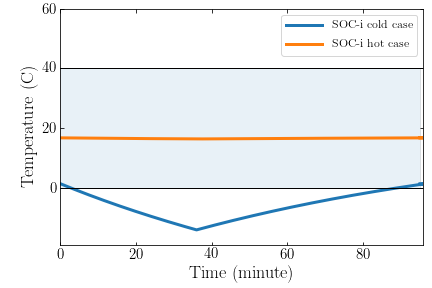
\includegraphics[width=0.45\textwidth, keepaspectratio]{figures/TempsPlot_SOCi-hotVScold.png} 
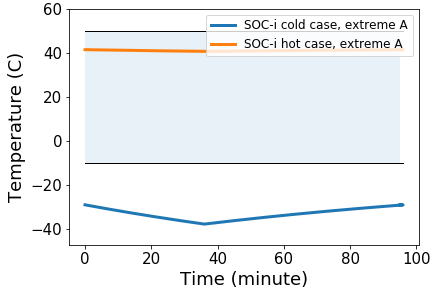
\includegraphics[width=0.45\textwidth, keepaspectratio]{figures/TempsPlot_SOCi-hotVScoldExtremeA.png} 

\caption{The impact of choosing extreme values of environmental conditions on Perun temperature,  
when assuming randomized satellite orientation (left), and with orientation that maximizes the temperature 
range between these so-called ``hot'' and ``cold'' cases (right). The temperature variation is compared to 
a typical battery operating temperature range (the blue horizontal band).  For hot case, there is no 
temperature variation with time because the assumed orbit has no eclipsed portion. 
\label{fig:SOCi1}}
\end{figure}


\section{Active temperature control \label{sec:active}} 

Given the allowed operating temperature ranges for satellite components (the most stringent requirement
comes from batteries, chosen here as 0--40 $^\circ$C for illustration), these results imply that 
low temperatures will be more worrisome than high temperatures. Motivated by this finding, we 
explored a model for active temperature control.




\subsection{A toy model for active temperature control } 

We developed a toy model for active temperature control that assumes an additional internal power 
dissipation whenever the satellite temperature drops below a pre-defined threshold. We investigated
cold case and three levels of power (2 W, 5, W, 10 W) that is applied whenever the temperature 
drops below 273 K (0 $^\circ$C). Results are shown in figure~\ref{fig:SOCi2}. 

Additional power can raise the satellite temperature by 5 to 11 degrees. The consumed power ranges
from 1.9 Wh to 4.3 Wh, and it is under the total available battery power (5.6 Wh for cold case and
$\eta_{cell}=0.2$; for hot, extreme case, it could be boosted to 18 Wh with $\eta_{cell}=0.3$). 
These results show that such an approach is a viable method for mitigating low temperatures.

\begin{figure}[t!]
\centering
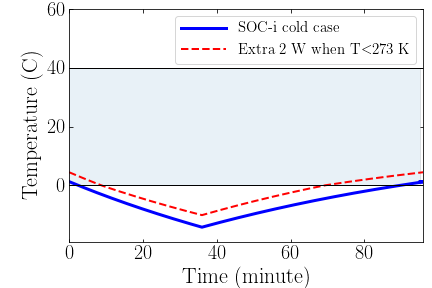
\includegraphics[width=0.3\textwidth, keepaspectratio]{figures/TempsPlotCompare_SOCi-cold-heated2.png} 
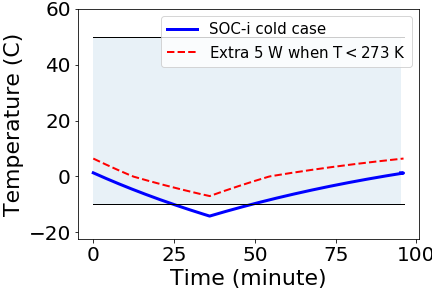
\includegraphics[width=0.3\textwidth, keepaspectratio]{figures/TempsPlotCompare_SOCi-cold-heated5.png} 
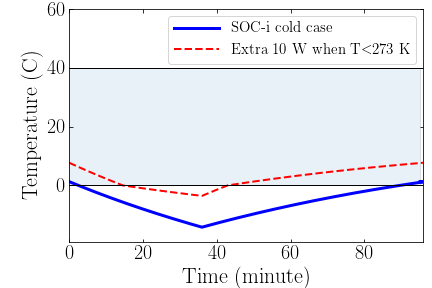
\includegraphics[width=0.3\textwidth, keepaspectratio]{figures/TempsPlotCompare_SOCi-cold-heated10.png} 
\caption{Illustration of the impact of active thermal control. A toy model assumes that whenever the satellite temperature
drops below zero $^\circ$C (273 K), an additional heating source with power of 2 W (left),  5 W (middle), or 10 W (right) contributes
to the heat balance. The blue lines correspond to the blue line in the left panel in figure~\ref{fig:SOCi1} (cold case) and the 
red dashed line is the corresponding temperature prediction with this additional heating power. The consumed power is about 
1.9 Wh, 3.4 Wh and 4.3 Wh, respectively (the total available battery power is 5.6 Wh). 
\label{fig:SOCi2}}
\end{figure}




\section{Conclusions \label{sec:conclusions}} 

We computed temperature variation with time for Perun satellite using a model with a single 
temperature that applies to the entire satellite surface at any given time, and a variety of input 
assumptions. 
 
We defined the so-called ``hot'' and ``cold'' cases and found that the low and high temperature 
extremes for a randomly oriented Perun satellite are $-$14 $^\circ$C and $+$17 $^\circ$C. When the 
satellite orientation is deliberately chosen to maximize the temperature extremes, the corresponding 
values are $-$38 $^\circ$C and $+$42 $^\circ$C. 

Within the model limitations, these estimates are accurate to within a few degrees. The results are 
sensitive to assumed specific heat, which we simply assumed to correspond to aluminum. 

Since it appeared that low temperatures will be more concerning than high temperatures,
we also explored a toy model for active temperature control that assumes an additional internal 
power dissipation whenever the satellite temperature drops below a pre-defined threshold. 
We found out that such an approach is a viable method for mitigating low temperatures.

Without more detailed and robust Perun orbit and orientation descriptions, this model cannot
be appreciably improved. Nevertheless, significant additional insight can be gained from Ansys
models that are capable of computing temperature field throughout the satellite body. For
external heat fluxes, values listed in Table~\ref{tab:inputflux} can be used but {\bf they need
to be corrected for different values of absorption coefficient ($\alpha$) for each surface 
material.} 

It would be prudent to first start with hot case because there is no temperature variation along
the orbit and thus much faster steady-state Ansys calculation can be utilized. Once that case is verified
to be in approximate agreement with the results presented here (in particular, we expect that
the mean external surface temperature of 17 $^\circ$C for random orientations should be reproduced
to within a few degrees), transient thermal analysis should be attempted for cold case. 



The latex source for this document, and the supporting python code, are publicly 
available\footnote{https://github.com/ivezic/CubeSats}. 



\vskip 0.2in 
\leftline{\bf References}
Gilmore, D. 2002, ``Spacecraft Thermal Control Handbook: Fundamental Technologies'', 2nd ed. Aerospace Press 

Hengeveld, D.W. et al. 2009, ``Hot- and Cold-Case Orbits for Robust Thermal Control'', Journal of Spacecraft and 
     \phantom{xxxxxx} Rockets,  Vol. 46, No. 6 

Jacques, L. 2009, ``Thermal Design of the Oufti-1 Nanosatellite'', Master Thesis, University of Liege

Kang, S-J. \& Oh, H-U. 2016, ``On-Orbit Thermal Design and Validation of 1 U Standardized CubeSat of STEP 
\phantom{xxxxxx}  Cube Lab'', 
        International Journal of Aerospace Engineering, Vol. 2016, Article 4213189

Kellens, A. 2018, ``Thermal design of the OUFTI-Next mission'', Master thesis, University of Liege
\end{document}

